\chapter{Introduction}
	\section{The Need For Spin Models}
	The study of statistical mechaincs arose due to the need to connect the physical descriptions
	of large particle systems in the macroscopic and microscopic realms. This is done by bridging 
	thermodynamic quantities (macroscopic) , such as temperature, with microscopic
	observables that fluctuate about some average. This is achieved using statistical methods and 
	probability theory. Applying the methods developed by statistical mechanics to various mathematical 
	models has given physicsts enormous insight into various physical phemoena and gives justification 
	to study these models in detail. 

	We begin by constructing a physical model, using a substance whose individual atoms are arranged 
	in a regular crystalline lattice. Furthermore, suppose that each atom in the lattice has a magnetic 
	moment which we call it's spin. In this picture, we also assume that these moments tend to align 
	with their neighbours\footnote{this assumption will be made concerete later} and an external 
	magnetic field $H$. We introduce a measurement parameter called the magnetization, which is simply 
	the global average of these spins.

	\begin{figure}[h]
		\centering
		\def\svgwidth{\columnwidth}
		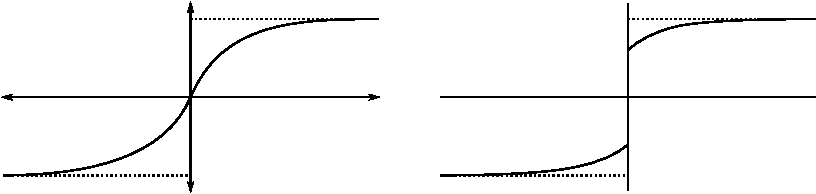
\includegraphics[width=0.8\textwidth]{chapters/images/chpt1-fig1.pdf}
		\caption{}
	\end{figure}


	Varying the external magnetic field, we can observe two distinct behaviours around $H=0$, called
	paramagnetic and ferromagnetic behaviour, first observed by Pierre Curie in 1895. In the first case, 
	as $H \rightarrow 0$, the global order (ie: spin alignment) is lost and the magnetization tends to 
	zero. In the ferromagnetic case, the local spin interactions are strong enough that the substance 
	maintains a global non-zero net magnetization. The value of this magnetization depends on the 
	direction in which the magnetic field approaches $0$. Thus, a ferromagnet displays 
	a \textit{spontaneous magnetization} $\pm M$ at $H=0$. This is a discontinuity in the magnetization,
	which corresponds to a \textit{first order phase transition}

	The observations by Curie also established that a temperature dependent transition occurs in 
	ferromagnetic materials, in which the material changes into a paramagnetic material. This transition 
	occurs at a well-defined temperature called the Curie Temperature. A goal of 20th century 
	thermodynamics was to be able to describe this phase transition using the framework of statistical 
	mechanics. 

	In 1920, Wilhelm Lenz introduced what is now called the Ising Model (a term coined by Rudolph 
	Peierls) to help understand that phase transition. The one-dimensional case was solved by 

	\section{Defintions for the Spin \texorpdfstring{$\ON{n}$}{O(n)} (Symmetric) Model}
		We begin the discusiion of the model by defining the system on which the model "lives". 

	\begin{ndefi}
		Let $d \geq 1$ and let $G = \rpth{V(G), E(G)}$ be a finite, non-oriented graph. The set of 
		vertices $\Lambda$ is defined to be a subset of $\Z^d$ (that is, $V(G) = \Lambda$, with 
		the coordinates $i = \rpth{i_1, \dots ,i_d} \in \Lambda $ being integers). We also 
		define the egdes of the graph $E(G)$ to be between the \textit{nearest neighbours} of $\Lambda$. 
		That is, pairs $\rpth{i,j}$ with $\norm{i-j}_1 = 1$. We denote nearest neignbours as 
		$\inprod{i}{j}$. 
	\end{ndefi}

	Throughout the remainder of this text, we shall call the graph $G = \rpth{\Lambda, E}$ a 
	\textit{lattice} and simply refer to it as $\Lambda$. We also remark that $\Lambda$ can also 
	be $\Z^d$ itself. This is referred to as the \textit{thermodynamic limit}. The need for this limit 
	will be made apparent later.

	Fixing $n \in N$, we have the \textit{single spin configuration} as 
	\[ \Omega_0 = \clpth{\sigma \in \R^n \ \mathrm{such \ that} \ \norm{\sigma}_2} = 1 \equiv \Sbb^{n-1}\]
	Following from this, we have a \textit{microstate}, often referred to as a 
	\textit{spin configuration}, on $\Lambda$ as 
 	\[ \Omega_{\Lambda} =  \Omega_0^{\Lambda} \]
	and in the thermodynamic limit $\Omega = \Omega_0^{\Z^d}$
	 
	For each $i \in \Lambda$, we call the random variable $\vectr{\sigma}_i: \Omega_{\Lambda} 
	\rightarrow \Sbb^{n-1}$ assigned to each point the lattice as the \textit{spin}. We add two special
	restrictions onto these spins: 
	\begin{itemize}
		\item That the spins themselves interact with their nearest neighbours
		\item This same interaction is invariant under a simultaneous rotation of the 
			entire configuration\footnote{The discussion of an external magnetic field will occur with 
			the Ising Model}
	\end{itemize}
	With these restrictions, we can then assume that only a function of the inner/scalar product of the 
	interacting spins contribute to the total energy of the system. We therefore arrive at what is 
	\textit{probably} the most important definition of the entire report

	\begin{ndefi}
		Let $U: [-1,1] \rightarrow \R$ (usually referred to as the \textit {potential function}) 
		and $\mathcal{H}_{\Lambda}$ be the Hamiltonian of an $\ON{n}$-symmetric model, over a lattice 
		$\Lambda$. We thus have
		\begin{equation}
			\mathcal{H}_{\Lambda} = \sum_{\inprod{i}{j}} U\rpth{\inprod{\vectr{\sigma}_i}
			{\vectr{\sigma}_j}}
		\end{equation}

		In particular, if we have $f(x) = -x$, we then have the definiton of the Hamiltonian for 
		the $\ON{n}$ (or $n$-vector) model
		\begin{equation}
		H_{\Lambda} = - \sum_{\inprod{i}{j}} \inprod{\vectr{\sigma}_i}{\vectr{\sigma}_j}
		\end{equation}
	\end{ndefi}

	We can now plug in different values of $n$ to get different models 
	\begin{itemize}
		\item $n=1$ gives the \textit{Ising Model}, with spins taking values in $\clpth{\pm1}$. The 
			discussion on this model is given below
		\item $n=2$, the spins lie along the circle with radius $1$ (hence $\ON{2}$ symmetric). This
			is called the \textit{XY Model} and is also central to the discussion. 
		\item $n=3, n \rightarrow \infty$ are called the \textit{Heisenberg Model} and 
			\textit{Berlin–Kac Spherical Model}. $n=4$ can be used as a "toy" model of the Higgs Sector.
	\end{itemize}

	\begin{ndefi}
		At inverse temperature $\beta \in [0,\infty)$, configurations are randomly chosen from the 
		probability measure $\mu$ defined as
		\begin{equation}
			\mathrm{d}\mu = \frac{1}{Z} \exp\rpth{{\beta H(\sigma_i, \sigma_j)}} \mathrm{d}\sigma
		\end{equation}
		where $Z$ is the normalization constant called the \textit{partition function}, given by

		\begin{equation}
			Z = \int_{\Omega_{\Lambda}} \exp\rpth{\beta H(\sigma_i, \sigma_j)} \mathrm{d}\sigma
		\end{equation}
	\end{ndefi}



